\apendice{Especificación de Requisitos}


\section{Diagrama de casos de uso}
En la Figura \ref{fig: diagrama_casos_uso} se muestra el diagrama de casos de uso del sistema, diferenciando entre las funcionalidades desarrolladas por el programador y aquellas que ejecuta el médico desde la interfaz final. 
\begin{figure}[h]
    \centering
    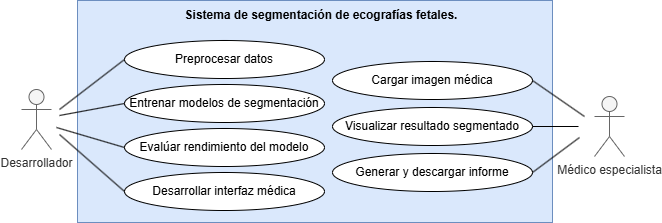
\includegraphics[width=1.1\textwidth]{img/diagrama_casos_usos.png}
    \caption{Diagrama de casos de uso.}
    \label{fig: diagrama_casos_uso}
\end{figure}

\section{Explicación casos de uso}
Esta sección presenta la explicación de los casos de uso del sistema. En cada tabla se resume de forma estructurada las principales interacciones entre los usuarios y el sistema, incluyendo su contexto, acciones implicadas y condiciones relevantes para su ejecución.

\begin{table}[!h]
	\centering
	\begin{tabularx}{\linewidth}{ p{0.21\columnwidth} p{0.71\columnwidth} }
		\toprule
		\textbf{CU-1}    & \textbf{Cargar imagen médica}\\
		\toprule
		\textbf{Versión}              & 1.0    \\
		\textbf{Autor}                & Eira Rodríguez Martín \\
		\textbf{Requisitos asociados} & RF-01 \\
        \textbf{Actor}                & Médico \\
		\textbf{Descripción}          & El usuario clínico selecciona e introduce en el sistema una imagen ecográfica fetal que será procesada para la segmentación.\\
		\textbf{Precondición}         & El usuario debe estar en la interfaz principal. \\
		\textbf{Acciones}             &
		\begin{enumerate}
			\def\labelenumi{\arabic{enumi}.}
			\tightlist
			\item El usuario hace clic en "Browse files".
			\item Se abre el explorador de archivos.
            \item El usuario selecciona una imagen valida.
            \item La imagen se carga y se muestra en la interfaz.
		\end{enumerate}\\
		\textbf{Postcondición}        & La imagen queda visible y lista para sementar. \\
		\textbf{Excepciones}          & La imagen no es válida o tiene un formato incorrecto. \\
		\textbf{Importancia}          & Alta \\
		\bottomrule
	\end{tabularx}
	\caption{CU-1 Cargar imagen médica.}
\end{table}

\begin{table}[!h]
	\centering
	\begin{tabularx}{\linewidth}{ p{0.21\columnwidth} p{0.71\columnwidth} }
		\toprule
		\textbf{CU-2}    & \textbf{Visualizar resultado segmentado}\\
		\toprule
		\textbf{Versión}              & 1.0    \\
		\textbf{Autor}                & Eira Rodríguez Martín \\
		\textbf{Requisitos asociados} & RF-02 \\
        \textbf{Actor}                & Médico \\
		\textbf{Descripción}          & El sistema genera la segmentación automática y la muestra junto a la original.\\
		\textbf{Precondición}         & Se ha cargado correctamente una imagen médica que corresponda a una ecografía del cerebro fetal. \\
		\textbf{Acciones}             &
		\begin{enumerate}
			\def\labelenumi{\arabic{enumi}.}
			\tightlist
			\item El sistema procesa automáticamente la imagen.
			\item Se ejecuta el modelo de segmentación.
            \item Se muestra el resultado en la interfaz.
		\end{enumerate}\\
		\textbf{Postcondición}        & El médico visualiza el resultado y puede interpretarlo. \\
		\textbf{Excepciones}          & Error en la predicción o visualización. \\
		\textbf{Importancia}          & Alta \\
		\bottomrule
	\end{tabularx}
	\caption{CU-2 Visualizar el resultado segmentado.}
\end{table}

\begin{table}[!h]
	\centering
	\begin{tabularx}{\linewidth}{ p{0.21\columnwidth} p{0.71\columnwidth} }
		\toprule
		\textbf{CU-3}    & \textbf{Generar y descargar el informe}\\
		\toprule
		\textbf{Versión}              & 1.0    \\
		\textbf{Autor}                & Eira Rodríguez Martín \\
		\textbf{Requisitos asociados} & RF-03 \\
        \textbf{Actor}                & Médico \\
		\textbf{Descripción}          & El sistema permite generar un informe médico en formato PDF con los resultados y datos del paciente.\\
		\textbf{Precondición}         & Debe haberse realizado la segmentación de una imagen. \\
		\textbf{Acciones}             &
		\begin{enumerate}
			\def\labelenumi{\arabic{enumi}.}
			\tightlist
			\item El usuario introduce los datos del paciente.
			\item El sistema genera el informe con la imagen original y la predicción.
            \item El usuario descarga el archivo PDF.
		\end{enumerate}\\
		\textbf{Postcondición}        & El informe queda guardado localmente. \\
		\textbf{Excepciones}          & Error al generar o guardar el archivo. \\
		\textbf{Importancia}          & Alta \\
		\bottomrule
	\end{tabularx}
	\caption{CU-3 Generar y descargar informe.}
\end{table}

\begin{table}[!h]
	\centering
	\begin{tabularx}{\linewidth}{ p{0.21\columnwidth} p{0.71\columnwidth} }
		\toprule
		\textbf{CU-4}    & \textbf{Preprocesar datos}\\
		\toprule
		\textbf{Versión}              & 1.0    \\
		\textbf{Autor}                & Eira Rodríguez Martín \\
		\textbf{Requisitos asociados} & RF-04 \\
        \textbf{Actor}                & Desarrollador \\
		\textbf{Descripción}          & El desarrollador prepara los datos de entrenamiento, generando máscaras.\\
		\textbf{Precondición}         & Disponibilidad de las imágenes. \\
		\textbf{Acciones}             &
		\begin{enumerate}
			\def\labelenumi{\arabic{enumi}.}
			\tightlist
			\item Se crean anotaciones de las imágenes.
			\item Se adaptan al formato COCO.
            \item Se generan las máscaras desde las anotaciones.
		\end{enumerate}\\
		\textbf{Postcondición}        & Los datos quedan listos para entrenar modelos. \\
		\textbf{Excepciones}          & Error en el formato de anotaciones o clases no encontradas. \\
		\textbf{Importancia}          & Alta \\
		\bottomrule
	\end{tabularx}
	\caption{CU-4 Preprocesar datos.}
\end{table}

\begin{table}[!h]
	\centering
	\begin{tabularx}{\linewidth}{ p{0.21\columnwidth} p{0.71\columnwidth} }
		\toprule
		\textbf{CU-5}    & \textbf{Entrenar modelos de segmentación}\\
		\toprule
		\textbf{Versión}              & 1.0    \\
		\textbf{Autor}                & Eira Rodríguez Martín \\
		\textbf{Requisitos asociados} & RF-05 \\
        \textbf{Actor}                & Desarrollador \\
		\textbf{Descripción}          & El desarrollador entrena modelos con los datos procesados utilizando PyTorch Lightning.\\
		\textbf{Precondición}         & Conjunto de datos preprocesado y modelo configurado. \\
		\textbf{Acciones}             &
		\begin{enumerate}
			\def\labelenumi{\arabic{enumi}.}
			\tightlist
			\item Se carga el conjunto de datos segmentado.
			\item Se define el modelo y los hiperparámetros.
            \item Se entrena con callbacks como \textit{early stopping}.
		\end{enumerate}\\
		\textbf{Postcondición}        & Modelo entrenado y guardado. \\
		\textbf{Excepciones}          & Fallos en entrenamiento. \\
		\textbf{Importancia}          & Alta \\
		\bottomrule
	\end{tabularx}
	\caption{CU-5 Entrenar modelos de segmentación.}
\end{table}

\begin{table}[!h]
	\centering
	\begin{tabularx}{\linewidth}{ p{0.21\columnwidth} p{0.71\columnwidth} }
		\toprule
		\textbf{CU-6}    & \textbf{Evaluar rendimiento del modelo}\\
		\toprule
		\textbf{Versión}              & 1.0    \\
		\textbf{Autor}                & Eira Rodríguez Martín \\
		\textbf{Requisitos asociados} & RF-06 \\
        \textbf{Actor}                & Desarrollador \\
		\textbf{Descripción}          & Evaluación del modelo con métricas como la precisión e IoU para valorar su desempeño.\\
		\textbf{Precondición}         & Modelo entrenado y conjunto de validación o prueba disponible. \\
		\textbf{Acciones}             &
		\begin{enumerate}
			\def\labelenumi{\arabic{enumi}.}
			\tightlist
			\item Se carga el modelo y los datos de evaluación.
			\item Se calculan métricas estándar de segmentación.
            \item Se comparan los resultados entre modelos entrenados.
		\end{enumerate}\\
		\textbf{Postcondición}        & Informa de métricas generado. \\
		\textbf{Excepciones}          & Métricas inconsistentes o mal calculadas. \\
		\textbf{Importancia}          & Media \\
		\bottomrule
	\end{tabularx}
	\caption{CU-6 Evaluar rendimiento del modelo.}
\end{table}



\begin{table}[!h]
	\centering
	\begin{tabularx}{\linewidth}{ p{0.21\columnwidth} p{0.71\columnwidth} }
		\toprule
		\textbf{CU-7}    & \textbf{Desarrollar interfaz médica}\\
		\toprule
		\textbf{Versión}              & 1.0    \\
		\textbf{Autor}                & Eira Rodríguez Martín \\
		\textbf{Requisitos asociados} & RF-07 \\
        \textbf{Actor}                & Desarrollador \\
		\textbf{Descripción}          & Implementación de una interfaz gráfica intuitiva que permita al médico subir imágenes, visualizar la segmentación y descargar el informe.\\
		\textbf{Precondición}         & El modelo de segmentación ya debe estar entrenado y disponible. \\
		\textbf{Acciones}             &
		\begin{enumerate}
			\def\labelenumi{\arabic{enumi}.}
			\tightlist
			\item Se diseña una interfaz adaptada al flujo clínico.
			\item Se realiza el testeo de usabilidad y funcionalidad.
		\end{enumerate}\\
		\textbf{Postcondición}        & Aplicación lista para uso clínico. \\
		\textbf{Excepciones}          & Problemas en la visualización o errores de compatibilidad. \\
		\textbf{Importancia}          & Alta \\
		\bottomrule
	\end{tabularx}
	\caption{CU-7 Desarrollar interfaz médica.}
\end{table}
\FloatBarrier
\section{Prototipos de interfaz o interacción con el proyecto}

La interfaz desarrollada para este proyecto tiene como objetivo principal facilitar el uso de la herramienta por parte del personal médico, ofreciendo una experiencia intuitiva y visualmente clara. 

En la Figura \ref{fig:subir_imagen} se muestra la forma de subir una imagen médica mediante el botón \textit{"Browse files"}.

\begin{figure}[h]
    \centering
    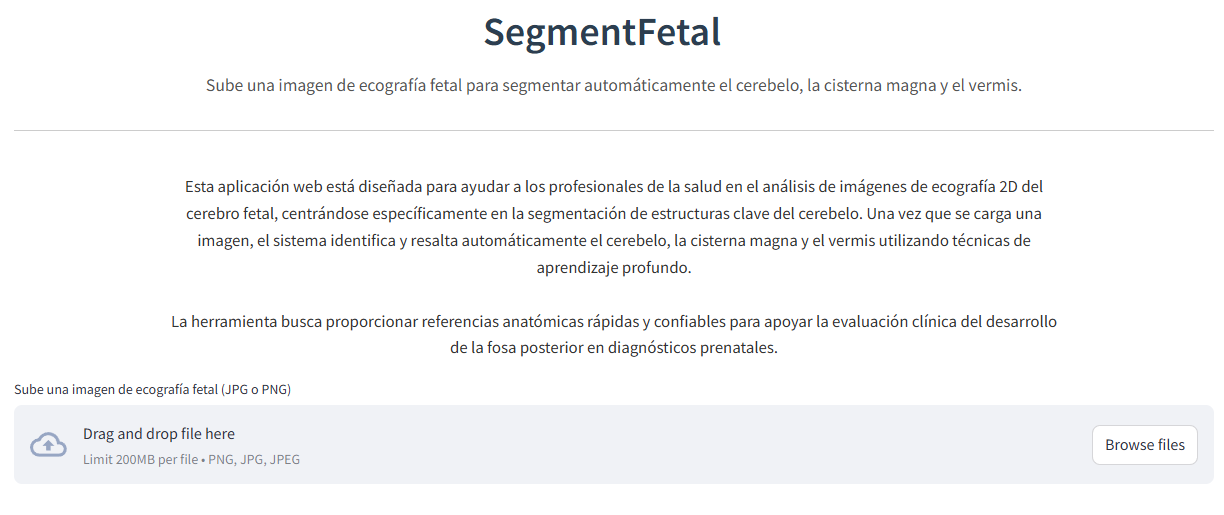
\includegraphics[width=1\textwidth]{img/interfaz_subir_imagen.png}
    \caption{Cargar imagen médica.}
    \label{fig:subir_imagen}
\end{figure}

La Figura \ref{fig:visualizar_segmentación} muestra cómo se visualizan la imagen original y la imagen tras la segmentación automática.

\begin{figure}[h]
    \centering
    \includegraphics[width=1\textwidth]{img/interfaz_visualización.png}
    \caption{Visualizar segmentación automática.}
    \label{fig:visualizar_segmentación}
\end{figure}

En la Figura \ref{fig: generar_informe} podemos observar la posibilidad de rellenar la información del paciente y generar el informe.

\begin{figure}[h]
    \centering
    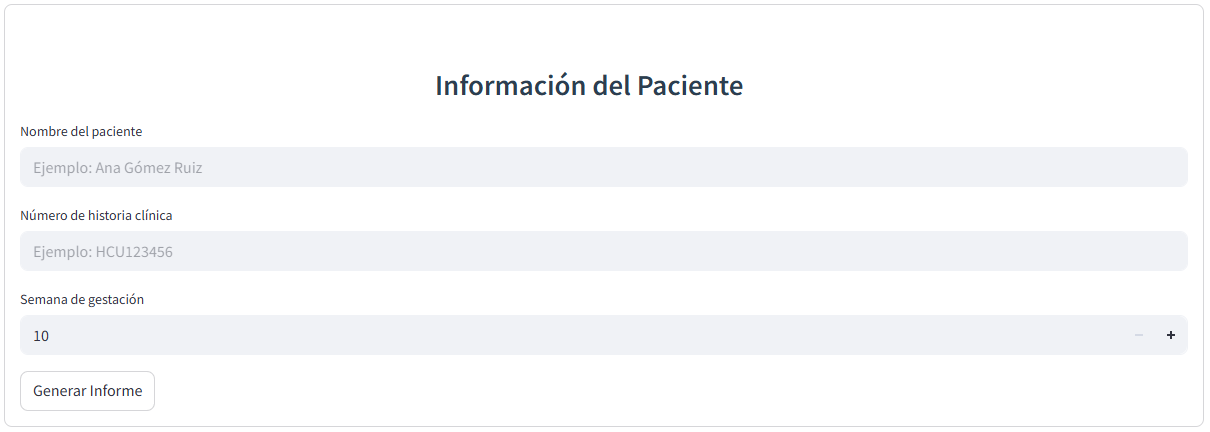
\includegraphics[width=1\textwidth]{img/interfaz_generar_informe.png}
    \caption{Generar informe.}
    \label{fig: generar_informe}
\end{figure}